%\chapter{Compact Object in Globular Clusters}
\chapter{Introduction}
\thispagestyle{fancy}


\section{Location, Location, Location}

Important in real estate, but also seems to be an important factor to take into account when studying compact objects in binary systems. It seems that, like with people, where you were born plays a role on your evolution. This seems to be true for cataclysmic variables (CVs), the kind of compact binary system that we will explore in more detail in the present work. Our goal is to try to understand the formation of these kind of systems when they are formed in a crowded and high density environment (like in a cluster of stars), and when you give them enough time to evolve and interact with other stars (like in a globular cluster).  

Now that we have defined our broad goal let's take a step back and explore in more detail what are compact objects, their different types, and the different ways they can interact with each other and other types of stars (Sec. \ref{sec:co}). That section will lead us to the discussion of where and how we expect to find them, and what can we learn by studying them in the different environment where they form (sections \ref{sec:gc}).

\section{Compact Objects or Stellar remnants}\label{sec:co}

Compact object, as their name suggest, are very massive and dense objects formed from the remains of a dying stars; hence their other name, 'stellar remnants'. They come in three main flavors, each following a different formation mechanism that is mainly determined by the mass of the progenitor star (ref.). The different types are neutron stars (NS), black holes (BH), and white dwarfs (WD). Besides these three, other possible exotic types of stars have been proposed; including quark stars, boson stars, and Thorne-Zytkow objects. These will not be discussed in this work as there is still a lack of observational evidence concerning their existence. The reader is refer to the following references to discover more about these particular kind of proposed stars. (Find references for exotic stars). 

On the three confirmed compact objects (neutron stars, white dwarfs and black holes), we will focus on the first two (NS and WD). They below to a class of object called "degenerate objects". These are object for which the supporting force comes from the degeneracy pressure of fermions\footnote{Fermions are particles with half-integer spin. They follow the Fermi-Dirac statistics, thus obey the Pauli exclusion principle. The consequence of the exclusion principle is that two fermions cannot occupy the same quantum state. This is the origin of the degeneracy pressure. }. In the case of a white dwarf the pressure is provided by the degenerate electron gas \citep{fowler_dense_1926}, and for a neutron stars, clearly, the neutrons cause the repulsive pressure (ref). 

The next subsection will list some of the characteristic for NS, and WD (both when they are found in isolation (sec~\ref{sec:wd} and~\ref{sec:ns}) or in a binary system sec~\ref{sec:cb}). Black holes will be briefly discussed for the sake of completeness. 


\subsection[White Dwarfs]{White Dwarfs}\label{sec:wd} 

White dwarfs are the most common end product in the evolution of stars. Around $90 \%$ will evolve to become one \citep{koester_white_1980}. This includes all main sequence stars \footnote{Main sequence stars are those that are burning hydrogen in their cores.} (MS) with a mass between $0.6$ and  $8$ M$_\odot$ \citep{koester_physics_1990}. The resulting white dwarf will have a mass between 0.3 and 1.4 M$_\odot$ \citep{prada_moroni_very_2009,chandrasekhar_maximum_1931}, the average mass being $\sim 0.7$ M$_\odot$ \citep{koester_physics_1990}. All this mass is contained in a radius of about $\sim 0.01$ R$_\odot$ \citep{kepler_structure_1995}. This are average values, but the mass-radius relation for a white dwarf is plotted in fig~\ref{fig:massrad}. If we take the mean values mentioned before this gives a mean density of $10^9$ kg$/$m$^3$ . This mass-radius relation will be composition dependent and it depends, for example, on the element dominiating the atmosphere composition \citep{hamada_models_1961}. About $80 \%$ of all white dwarfs have hydrogen-dominated atmospheres (spectral type DA), but there exists a second class where helium dominates the atmosphere composition (spectral types D0, DB, DC, DZ and DQ)\citep{wickramasinghe_magnetism_2000,koester_physics_1990}. White dwarfs are also known to be magnetic. Surface magnetism ranges from about $10^5$ to $10^9$ G \citep{suh_mass-radius_2000}. Isolated magnetic whit dwarfs represent $\sim 5 \%$ of all WDs. See \cite{wickramasinghe_magnetism_2000} for a review on magnetism in WDs and for more details on the physics of white dwarfs the reader is referred to \cite{koester_physics_1990} and \cite{kepler_structure_1995}.

\subsection{Neutron Stars}\label{sec:ns}

Neutron stars, first proposed in 1934 by Baade and Zwicky,  are stars where the sustaining force against gravity comes from  the degeneracy pressure between neutrons \citep{baade_cosmic_1934}. These stars are produced from the gravitational collapse of a massive star (> 8 M$_\odot$)(ref for mass range) at the end of its life. The type II supernova produced by this collapse, leaves behind a dense and massive core. A core of $\sim 12$ kilometers in radius (ref), but up to $\sim 2$ M$_\odot$ (this limit being model dependent. See \citep{lattimer_neutron_2007}). For comparison with white dwarf a sample mass-radius relation for a NS (red) is plotted along with that of a white dwarf (blue) in fig~\ref{fig:massrad}. Like WDs, neutron stars are also know to show magnetism. They have an average magnetic field strength of $<B>\sim 10^{14}$ G \citep{beskin2015magnetic}. There also exist some neutron stars with unusually high strong magnetic fields ($\text{B}\sim 10^{14} - 10^{15}\text{ G}$) and are called "magnetars" \citep{duncan_formation_1992}. For a review on magnetic fields in neutron stars see \cite{reisenegger_magnetic_2005}. 

Neutron stars are mainly composed of neutrons and a thin atmosphere of a few cm of hydrogen or helium (ref for NS atmosphere models). We have come a long way since the first proposition of their existence, but there is still a lot of  uncertainty concerning their interiors and a lot of existing conflicting models \citep{lattimer_neutron_2007}. Since we have had observational evidence on their existence (ref PSR B1919+21) efforts have been done to constrain the different models. Figure~\ref{fig:nsmod} shows a visual summary of some of the different models proposed. There are many ways that we can observationally constrain these models, spectroscopy being one of them.

\begin{figure}[]
        \centering
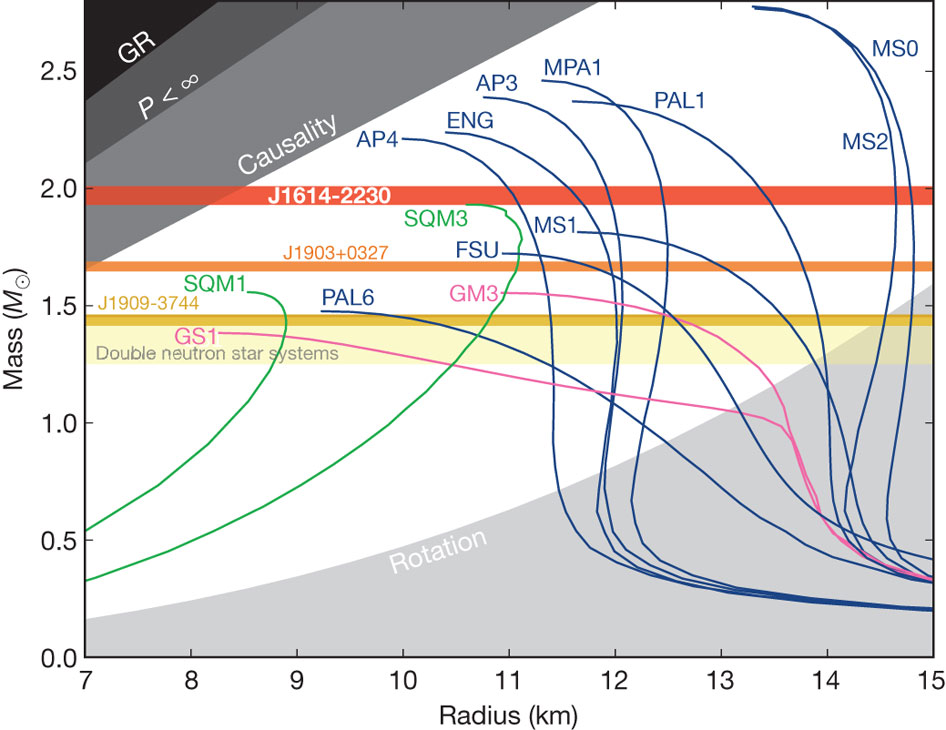
\includegraphics[scale=.3]{assets/images/es.jpg}
\caption{The plot shows non-rotating mass versus physical radius for several typical equation of states.  Blue, nucleons; pink, nucleons plus exotic matter; green, strange quark matter from (doi:10.1038/nature09466)}
\label{fig:nsmod}
\end{figure}

\subsection{Black Holes}\label{sec:bh}

Black holes are the fate of collapsing matter when no force, including the degeneracy pressure of neutrons, is not enough to repel gravitational attraction. Black holes,  like neutron stars and white dwarfs, can be the result of the collapse of a single main sequence star. Stars with an initial mass $\gtrsim  20$ can end up as a black hole \citep{heger_how_2003}, but the initial mass is not the only factor that comes into play. For example, the formation of the black hole will depend also on the metallicity of the star as well as the initial mass. See \cite{heger_how_2003} and \citep{brown_evolution_2000} for details on the evolution of high mass stars and the different formation path leading to a black hole from a single collapse star. 

To compare the physical characteristic of a black hole to other compact objects we can define the gravitational radius or Schwarzschild radius of a black hole. This is the radius to which a given mass needs to be reduced to get a escape velocity equal to the speed of light. This translates to:

%
%\begin{equation}
%        \frac{m c^2}{2} = \frac{G M m}{r} \\
%                \end{equation}
%solving for r we get:

\begin{equation}
                r = \frac{2 M G}{c^2}
\end{equation}

An estimate of the lowest mass of a black hole is the maximum possible mass for a neutron star, this is $\sim 3 \text{M}_\odot$ \citep{rhoades_maximum_1974}. With the formula above we can get a rough estimate on the size of a stellar mass black hole. A mass of 3 M$_\odot$ and the formula above gives an equivalent Schwarzschild radius of about 9 km. 


\begin{figure}
                \centering
                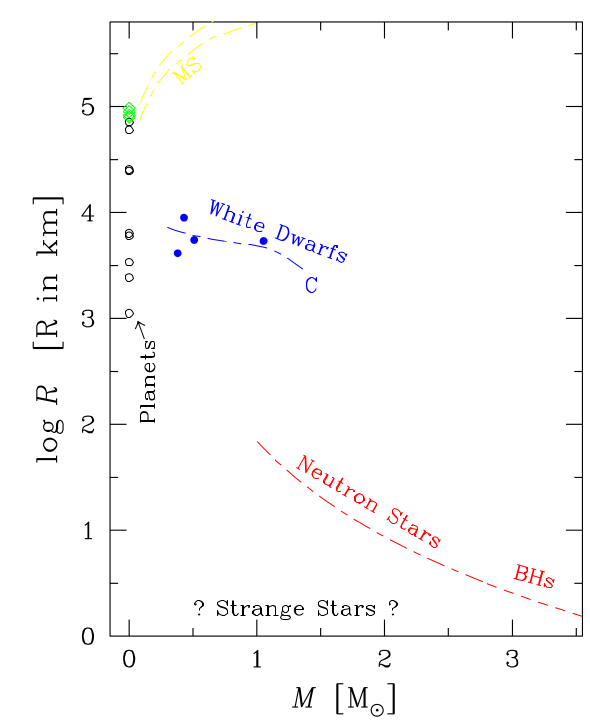
\includegraphics[scale=0.3]{assets/images/mass-radius.png}
                \caption{Mass-radius relation for different objects \citep{de2008stars}.}
                \label{fig:massrad}
\end{figure}

\section[Compact Binaries]{Compact Binaries}\label{sec:cb}

Compact binaries are those binaries where at least one of their components is a compact objects (WD, NS or BH). In this section we will start by discussing some of the basic concepts of binary evolution, follow by a discussion on mass exchange between binaries,  and finished by looking in more detail some specific examples of compact binaries that are relevant to this study.   

\subsection{The Gravitational Potential}

The total potential of a binary system is the sum of the gravitational and the rotational potential. To get an analytical solution we can assume a model in which the resulting disturbing potential is due to the presence of two point masses, M$_1$ (or the primary) and M$_2$ (also called the secondary). Moreover, we assume a co-rotating Cartesian reference frame (x,y,z) with origin at the primary M$_1$; whose x-axis is is in the direction joining the two point masses; and the z-axis is perpendicular to the orbital plane. The total potential at an arbitrary point P(x,y,z) then reads:

\begin{equation}
        \Psi = - G \frac{\text M _1}{\sqrt{x^2+y^2+z^2}} - G \frac{\text M _2 }{\sqrt{(R - x)^2 + y^2 + z^2}} - \frac{\omega^2 }{2}  \left [ (x- \mu R )^2  + y^2 \right ]    
        \label{eq:pot}
\end{equation}

where G is the gravitational constant, R represents the separation between the point masses, and $\mu = \text M _2/(\text M _1 + \text M _2)$. We further assume that the binary orbit is Keplerian, thus the orbital frequency is given by:

\begin{equation}
        \omega ^2 = G \frac{\text M _1 + \text M _2}{R^3}
        \label{eq:roche}
\end{equation}

Taking into the account the assumptions the surfaces generated by eq~\ref{eq:pot} are called \emph{Roche Equipotential}\footnote{We are neglecting here the radiation pressure from the stars. For more details on Roche Potentials Including Radiation Effects see \cite{schuerman_roche_1972}}. Fig~\ref{fig:roche} such such equipotential surfaces (x,y plane). Of special interest are two regions on the graph:
\begin{itemize}
        \item The inner Lagrangian point \textbf{L$_1$}. This is where all the forces cancel out. 
        \item Critical or \textbf{Roche lobe}. The surface that have the potential equal to the L$_1$ potential. 
\end{itemize}

The Roche lobe has the property that inside the lobe of an object, any material will be gravitationally bound to that object. With these knowldege we can classify binary systems in three groups:

\begin{enumerate}
        \item \textbf{Detached systems}. If the volumes of both components are significantly smaller than their Roche lobe. 
        \item \textbf{Semi-detached systems}. Where one of the components fills its Roche lobe.
        \item \textbf{Contact systems}. Where both components appear to fill their respective Roche lobes. 
\end{enumerate}

This classification scheme was first suggested by \citep{kopal_classification_1955} and developed in detail in a comprehensive monograph in 1959 \citep{kopal_close_1959}. 

\begin{figure}[]
        \centering
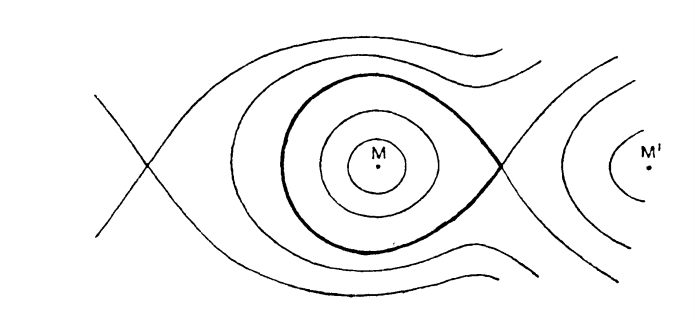
\includegraphics[scale=.3]{assets/images/kopalroche.png}
\caption{Geometry of the Roche surfaces. The Roche lobe is mark in bold font \citep{kopal_close_1959}.}
\label{fig:roche}
\end{figure}



\subsection{Binary Evolution}

In this work we are mostly interested in the formation of semi-detached compact binary systems. In this section we briefly explore a possible scenario for its formation. 

These kind of systems can be formed from two previously detached MS stars binaries that evolve in different timescales due to their different mass. This can be seen noticing that the luminosity, L, indicates the rate of consumption of nuclear fuel; and the nuclear fuel repository is proportional to the mass, M. This gives us a rough estimates of the nuclear timescale of a star given by:

\begin{equation}
        \tau \propto \frac{ M 6 \times 10^{18} \text{ergs g}^{-1}}{L}
\end{equation}

Where L is the luminosity, M is the mass,  and $6\times 10^{18} \text{ergs g}^{-1}$ is the energy release fusing a gram of hydrogen to helium. Moreover, with the mass-luminosity relation $ \text L / \text L _\odot = \left  (M / \text M _\odot \right )^\alpha $, where $\alpha \gtrsim 3$ (ref. missing), we can conclude that in a system starting with two detached main sequence stars, the more massive one will leave faster the main sequence and finished as a compact object (depending on its mass). This will leave a binary system with a compact object and a evolved main sequence star. The old main sequence star in the binary as it continues evolves will expand and fill its Roche lobe, allowing for accretion into the compact object to happen.  The process is more complex and, among other things, depends on the initial mass of both stars and initial binary separation. For example, a binary system starting with a 2 M$_\odot$  and  a 1 M$_\odot$ star can produce a white dwarf accreating from a late-type main sequence star \citep{kippenhahn_entwicklung_1967,de_loore_structure_1992}. A system starting with a 15 M$_\odot$ and 2 M$_\odot$ will become a neutron star accreting from a low mass main sequence star \citep{heuvel_late_1976}. In the case of starting masses of 20 $M_\odot$ + 8 $M_\odot$ this can produce a neutron star (or black hole) accreting from a high mass main sequence star \citep{heuvel_late_1976}. The details on the evolution of close binaries can be found in \cite{postnov_evolution_2014}.and \citep{de2008stars}

%\cite{paczynski_evolutionary_1971}.
% Parameters governing the specific orbital angular momentum of ejected matter, the common envelope and spiral-in phase, the asymmetric supernova explosion and the stellar evolution of the naked helium star all have a large impact on the exact evolution

In the next section we will see in some detail how the accretion can take place once the compact binary is formed due to stellar evolution of their constituents. 

\subsection{Accretion}

As mentioned before if one of the binaries fills its Roche lobe, material can flow via the L$_1$ point to the other star. This is what constitutes a semi-detached binary system. It would be a semi-detached compact binary if at least one is a compact object. Here we look in more detail the nature of the accretion in such a system where a compact object (primary) accreates from a main sequence star via Roche lobe overflow. 

In the Roche overflow scenario we have incoming gas from the secondary star. After it passes thought the L$_1$ point we assume a ballistic behaviour completely governed by the gravitational potential of the compact object. This is justified by the fact showed by \cite{lubow_gas_1975} that the stream is supersonic and we can ignore pressure. We can also assume that the incoming speed must be small. This is safe to assume if the accretion is due solely to overflow of the lobe and thus the velocity is in the order of the sound speed at the atmosphere of the secondary star. This speed ($\sim 10 $km/s reference missin) is much slower than the orbital speed of the binaries,  and lower than the velocities acquire during the fall. This simplification means that we can treat the Roche lobe as a zero velocity surface. Meaning that the motion of the gas can be approximated as the trajectory of a test particle release from rest with an initial angular momentum from L$_1$. This creates an elliptical orbit of the stream around the primary star (fig~\ref{fig:roche}~a). As the gas flow continues it will impact itself. This causes the flow to modify its orbit to that of the lowest energy at an specific angular momentum (we assume angular momentum is conserve). Of course the orbit of lowest energy at a given angular momentum is a circular one (see fig~\ref{fig:roche}~b). This creates a ring around the compact object.  We can estimate the radius of this ring by again invoking the assumption that no angular momentum is loss in the process. The angular momentum at L$_1$ would be given by  R$_{L1}$  V$_{orbit}$ (where R$_{L1}$ is the distance from the secondary to L$_1$). Knowing that $\omega = (2 \pi)/\text{Period}$ and equating the angular momentum at $L_1$ to the angular momentum of a Keplerian orbit at $R_{ring}$ we get:


\begin{equation}
        \frac{R_{ring}}{R} = \left ( \frac{\text R _{L1}}{R} \right ) ^{\frac{1}{4}} (1+q)
\end{equation}

where I used eq~\ref{eq:roche} to simply the answer by canceling some constants. This is called the \emph{circulation radius}. After a ring is formed (fig~\ref{fig:roche}~b), as first indicated in \cite{lynden-bell_evolution_1974}, any viscous processes will cause the ring to spreads to conserve angular momentum (fig~\ref{fig:roche}~d) The nature of these viscous torque won't be discussed here. For a review on the topic see \cite{frank_accretion_2002} and \cite{verbunt_accretion_1982}. It is only left to say that Roche lobe overflow is not the only type of accretion, for example wind accretion. In this work, unless otherwise stated, accretion will mean accretion by Roche lobe overflow. See the references cited above for more detail on other type of accretion. \\


Now that we studied briefly accretion and see how it can happen in semi-attached binaries, in the next section we will discuss two specific examples of this happening. One where the accretion is onto a white dwarf (Cataclysmic Variable), and the other where the accretion is onto a neutron star or a black hole (X-Ray binaries). 


\begin{figure}[]
        \centering
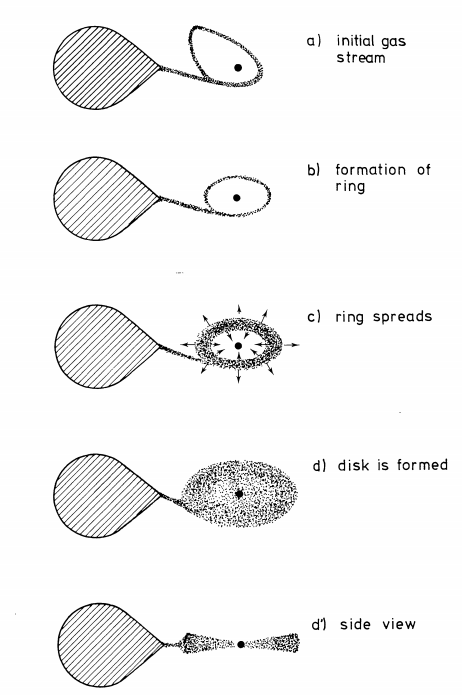
\includegraphics[scale=.3]{assets/images/accretiondisk.png}
\caption{Schematic illustration of the formation of an accretion disk around a compact binary \citep{verbunt_accretion_1982}.}
\label{fig:roche}
\end{figure}


%\FloatBarrier
\subsection{Cataclysmic Variables (CVs)}

Cataclysmic variables are semi-detached binary system comprised of a white dwarf (primary star) and typically a low mass main sequence star with a typical period in the range of 1-10 hrs (ref for period). CVs are generally classified into two groups. Magnetic CVs and nonmagnetic CVs (B < 0.01 MG). Magnetic CVs constitute about $25 \%$ of the CV population \citep{balman_x-ray_2012}. 

CVs can be observed in many wavelengths. This includes radio observation of jets \citep{nova_jets_2008,coppejans_novalike_2015}, optical and UV observation of the accretion disks \cite{1994ASPC...54...61K}, and X-rays ($\sim 0.5-2.5 keV$) from the infalling plasma onto the white dwarfs \citep{kuulkers_x-rays_2006}. As their name suggest these are very variable systems (specially the nonmagnetic CVS). These variabilities are due either by instability on the accretion disk, referred to as dwarf nova \citep{osaki_accretion_1974}, or unstable burning of hydrogen at their surface, called nova \citep{starrfield_thermonuclear_2016}. We will discuss in some detail the outburst caused by these instabilities, and the nature of the magnetic CVs by presenting the classification of CVs and exploring the taxonomy of these objects.  

\subsubsection{Classical Novae (CN)}

When the surface of an accreting white dwarf becomes hot enough ($\sim \times 10^8$ K \cite{starrfield_thermonuclear_2016}), nuclear fusion can take place and a thermonuclear runaway happens. This creates a violent explosion capable of ejecting material (mean mass of $\sim 2 \times 10^{-4} \text M_\odot$) at high velocities ($\sim 10^2 - 10^3$ km s$^{-1}$) \citep{gehrz_nucleosynthesis_1998,shara_recent_1989}. These outburst are fairly easy to detect since they cause a substantial increase in brightness (typically $\sim 12$ magnitudes \cite{shara_recent_1989}). A CV observed erupting in such a way is classified as a \emph{classical nova (CN)}. Classical novae are seen to erupt only one. If a previously recognized CN erupts again as a CN they are called recurrent novae. 

%Classical novae are the most violent non-destructive eruption observed from a CV, but not the only one. Another kind of instability can cause violent outburst in a CV and gives the name to the second type of non-magnetic CVs, dwarf novae. 

\subsubsection{Dwarf Novae (DN)}

A dwarf nova outburst is caused by instabilities in the accretion disk. This is predicted to happened in non-magnetic CVs with low accretion rates \citep{osaki_accretion_1974}. CVs that show these outbursts are classified as dwarf nova. The outburst from a dwarf nova is not as violent as the one from a classical novae. The magnitude change is only of about 2-5 , and no material is ejected. They also, unlike classical novae, are periodic in nature on times scales of weeks to years depending mainly on the accretion rate \citep{shara_recent_1989}. Probably the best know example of a dwarf nova is the variable star SS Cygni \cite{cannizzo_study_1998}. 

\subsubsection{Novae-like (NL)}


Another classification of white dwarfs is the novae-like. They are CVs that seem to have stable accretion, thus not undergoing dwarf novae outburst and having a bright stable disk. They represent the 'non-eruptive' CVs.

%\subsubsection{Magnetic CVs}

%These are CVs for which the magnetic field is strong. The actual definition is a bit more complex involving synchronization of orbit and rotation, and modulation of X-rays; but we don't need to know the details now. The main idea is that in the presence of a strong magnetic field the accretion flow can be disrupted. This disruption can be partial or complete. This then gives rise to a subdivision of these objects: Polars and Intermediate Polars.  They both share some characteristics. In both type of systems seem to be very variables (other of magnitudes and ref for this). They also share some spectral properties, the most noticeable one being the presence of Helium II. This is due to the ionized accreting plasma. 

\subsubsection{Polars}

Polars are CVs with a strong magnetic field. The value of the magnetic field is usually between 20 MG to 230  MG \citep{balman_x-ray_2012}. The field in polars is so strong that it couples to the field of the donor and forces the WD to corotate with the binary. The presence of the strong magnetic field also disrupt the accretion disk. In the case of Polars the accretion flow is redicted so it takes place at the magnetic pole guided by the magnetic field lines. This causes X-ray radiation and strongly polarized cyclotron radiation from IR to UV wavelengths \citep{cropper_polars_1990}. This polarized emmision is the reason for the name Polars \citep{krzeminski_extremely_1977}. The polarization was the first clue on the magnetic nature of these type of systems. It was first discovered for AM Herculis (AM Her), now the prototype polar CV (\cite{tapia_discovery_1977}). Polar systems are often referred to as AM Her-like system. This kind of systems represent $63 \%$ of the magnetic CV population \citep{balman_x-ray_2012}.

\subsubsection{Intermediate Polars (IPs)}

Intermediate polars are the second kind of magnetic CVs. In this type the magnetic field is weaker ($\sim 1-20 MG$). The weaker strength of the magnetic fields means that the accretion disk is not entirely dominated by the magnetic field, and the system is asynchronous, so the WD does not corotate with the binary. This kind of systems represent $37 \%$ of the magnetic CV population \citep{balman_x-ray_2012}. An extensively studied member of this class is DQ Her. DQ Her is somethings refer as a subclass of IPs (IPs with period $\lesssim 120 $ s), or even as a synonym for IP \citep{patterson_dq_1994,warner_cataclysmic_2003}.  


Should I include AM CVn? %\citep{solheim_am_2010}

%\subsection{Low-Mass X-Ray Binary}
\subsection{X-Ray binaries}

X-Ray binaries are a subclass of compact binaries where the accretor is either a neutron star or a black hole. They can be classified into two regimes depending on the type of the donor star. If the donor or secondary is a late-type star it is called, Low-mass X-ray binary; if it is an early-type star they are called high-mass X-ray binary.

\subsubsection{Low-mass X-Ray Binaries}

Low-mass x-ray binaries (LXMBs) are Roche-lobe overflow binary stars consisting of a neutron star or a black holes accreating from a low-mass ($\lesssim 1.5 \text M_\odot$) donor. The donor can be a main sequence star or even a white dwarf \citep{tauris_formation_2006}.

In the case of a LMXB, since the accretor (NS or BH) has a higher mass than the white dwarf in a CV, the energy release in the accretion process is higher. This means that we get more powerful X-ray radiation from LMXB (up to $\sim 10 \text keV$) \citep{tauris_formation_2006}. The period can range from 11 minutes to 17 days, and like CVs they can show magnetism ($\sim 10^9 \sim 10^{11} \text G$). (Do I use ibid. or cite again?). 


\subsubsection{High-mass X-Ray Binaries}

High-mass X-ray binaries (HMXB) are the second class of X-ray binaries. In the case of an HMXB the donor star is a young early-type main sequence star. This usually means a O or B spectral type with a mass $> 10 \text M _\odot$ \citep{tauris_formation_2006}. Contrary to the LMXB the accretion is not entirely due to Roche overflow, it can be due to the high velocity winds produced by the donor star. And also unlike the LMXB this systems tend to show stronger magnetic fields and stronger X-ray radiation (ibid.)

\subsection{The secondary stars}

\begin{comment}
The detailed study of the secondary stars in CVs can be on its own the sole topic of a thesis. Here we limit the discussion for late-type stars.  This is justified by the fact that we will be studying CVs in globular clusters. Globular clusters, as we will see in the next section, are very old clusters of stars, so the most common stars in the cluster are expected to have relatively small mass (Do i need to cite this). In fact for NGC 6397, the globular cluster studied in this work, the turnoff mass~\footnote{the turn off mass is the maximum mass on the main sequence. This can serve as a rough estimate of the maximum mass of main sequence stars in a globular clusters.} is $0.77 M_\odot$ \citep{de_marco_spectroscopic_2005}. 

Late-type stars can be a term a bit ambiguous, but in this report the term will exclusively refer to K and M type stars. Let's look at them in more detail.  

\subsubsection{K stars}

Search for good reference for info. They are discussed in Natalie's thesis. Include specta?


\subsubsection{M stars}

Search for good reference for info. Include specta? \\



With the discussion of the secondary stars we end our discussion on compact objects and binaries. In this section we learned what compact objects are and explored two specific types of accreting binaries, LMXB and CVs. We briefly mentioned the characteristics of an LMXB, and then focused on the CVs. We studied the rich nomenclature of CVs, and the different types of CVs based on their outburst and magnetic properties. But I must say that I have only touch the surface of this ample topic. The following references are valuable sources for the avid reader that wish to know more about the subject. The first good source of information is Warner's book \emph{Cataclysmic Variable Stars} \citep{warner_cataclysmic_2003}, an essential reference for this topic. Another good reference at a lower level and easier to read is \cite{hellier_cataclysmic_2001}. 

A review that deals with the evolution of LMXB and CVs (the two only binaries mentioned here) is \cite{patterson_evolution_1984}. Another one that don't limit the discussion to white dwarfs and neutron star is the book \cite{frank_accretion_2002}. The book extends the discussion to all the compact objects (including black holes) and discussed the physics of the different models of accretion besides Roche overflow. \\ 

Now that we have a better idea about compacts objects, specially about CVs, the next sections will be about where can search for compact binaries, and how. \\ 

Meyer & Meyer-Hofmeister (1981, 1982, 1983) firstly discussed the physical mechanism responsible
for dwarf nova outbursts which is connected with the thermal instability of the disc which occurs in the
temperature range corresponding to the ionization of hydrogen. Soon after Smak (1984a,b) extended the
study of such a mechanism. The details are summarized by Smak (2002) as follows.
From 2008ChJAS...8..237G   Cataclysmic Variables: A Review Giovannelli

Dwarf novae belong to the class of nonmagnetic cataclysmic
variables in which the magnetic field of the white dwarf is too
weak to disrupt the accretion disk, so that the disk can extend
close to the surface of the white dwarf 

%(see Warner 1995 for a review of dwarf novae).
\end{comment}

\section{Globular Clusters}\label{sec:gc}

Globular clusters (GCs) are very old and dense gravitationally bound group of stars. Their age is generally around 10 Gyr \citep{meylan_internal_1997} and typically contain $\sim 10^6$ stars \citep{knigge_cataclysmic_2012}. Due to their age we expect to find compact objects, and the high density environment is ideal for the formation of compact binaries. The search for these compact binaries have been fructiferous leading to the detection of X-ray binaries (\citep{}citation) and Cataclysmic Variables (\citep citation) in several globular clusters. But still the formation and evolution of these kinds of binaries is still not completely understood, and many uncertainties remain. Of special interest for this project are the cataclysmic variables in globular clusters. In the next subsection we will make a brief overview on the current knowledge on the subject and state the current open questions that we mean to address in this project. 

%dominating the dynamics of the clusters, they are home to a significant fraction of compact binaries.
%The formation and evolution of these kinds of binaries is still not completely understood.

%Old cluster or stars. Their age means that we expecdt a lot of death star. Perfec to search for comact obejct. A nother advanted is the know distance and age. We  

%As we saw. We expect them to form in high density envrioment. Revew 
%
%Know distance for example. 

\subsection{CVs in Globular clusters}\label{sec:cogc}

Cataclysmic Variables are tracers of the dynamical evolution in globular clusters. Their number and spatial distribution can give us a clue on the past of the globular cluster, and help us constraint models of stellar and dynamical evolution. CVs are expected to be the most abundant compact binary based on the fact that white dwarf is the most common fate of stars. Theoretical modeling predicts $\sim 100CVs$ in a given GC \citep{ivanova_formation_2006}.  They are expected to form two distinctive groups based on their formation mechanism, primordial CVs and dynamically formed CVs \citep{hut_binaries_1992}. Primordial are those CVs that formed from primordial binaries that didn't get destroyed through a physical collision in the cluster.The dynamically formed CVs are those formed via dynamical encounters with other members in the cluster. This includes tidal capture, exchange interactions and collision events. For example a dynamically formed CV can formed thought the tidal capture of an MS by a WD, or by a system resulting from the collisions between a red giant and a MS star \citep{ivanova_formation_2006}. 

The two expected formation mechanism clearly raises the question \textbf{Where are all the primordial CVs?}. The number can be theoretically predicted ($\sim 37 \%$ of all CVs in a GC \citep{ivanova_formation_2006}), but we need observational evidence to constraint the theoretical models. This still remains the case. The dense environment in which they form and the possibility that CVs are formed through dynamical interaction can result in a differentiation of the binary population from the galactic field population. For example, the result of these dynamical processes is that in the dense cores of GCs, binaries are strongly depleted and their period distribution is expected to be different from that of a field population \citep{ivanova_evolution_2005}. So the questions becomes, \textbf{What is the period distribution of CVs in Globlular Clusters}. In the galactic field the period distribution have been well studied. The period of CVs in the field is governed by magnetic braking ($\text P _{orb} \gtrsim  3 \text h$), and gravitational radiation ($\text P _{orb} \lesssim 2 h$) (ref for period gap). The period distribution in GC is still not well understood mainly due to lack of observational data. There are only 15 CVs with know periods from a small sample of 5 globular clusters (Should I cite all studies or can I cite a paper with all of them like  \cite{knigge_cataclysmic_2012}). Another difference between fields and GC CVs that have been proposed is that CVs in GCs tend to be primarily magnetic in nature \citep{grindlay_magnetic_1999}. This will explain the lack of observed dwarf novae outburst in CVs (ref) and the high X-ray luminosity of GC CVs, compared to fields CVs \citep{verbunt_cataclysmic_1997}. However data is scarce to support that argument and the questions remain: \textbf{Are globular clusters in CVs mainly magnetic in nature and where are all the dwarf novae?} \\

With the questions mentioned above in mind, in this project we studied the population of Cataclysmic Variables in an specific nearby globular cluster, NGC 6397. The next section describes the most important characteristic of NGC 6397 and the previous studies done regarding its compact binary population. 


%Theoretical models say that  only 25 per cent of CVs were formed in binaries that would become CVs in the field. \citep{ivanova_formation_2006}. 
%Another aspect in which the GC CVs can be different than the field cvs is magnetism. 
%nonmagnetic CVs produce an optically thick boundary layer, saturating their X-ray emission (Patterson & Raymond 1985).

\subsection{NGC 6397}

NGC 6397 is the closest (2.4 kpc) core collapse\footnote{Core collapse are clusters showing a power-law slope in their surface brightness profile near the center due to the gravothermal instability \citep{antonov_solution_1962,lynden-bell_gravo-thermal_1968,lynden-bell_consequences_1980}. In contrast to other isothermal sphere models showing a more flatten brightness profile in the center (e.g. \cite{king_structure_1966})} globular cluster \citep{harris_catalog_1996,mclaughlin_resolved_2005}.  The center of the cluster is located at RA(J2000): $17^h \, 40^m \, 42.09^s$  and Dec(J2000): $-53^\circ \, 40'\, 27.6"$ \citep{harris_catalog_1996}. Due to its proximity NGC 6397 have been extensively studied in different  wavelengths. The observation by \cite{cool_discovery_1993} with the ROSAT instrument was the first one to detect X-rays sources in NGC 6397. This was followed by a photometric study with the Hubble Space Telescope wide field and planetary camera confirming the first three CVs candidates in NGC 6397 \citep{cool_discovery_1995}. Since then observations with Chandra \citep{grindlay_chandra_2001,bogdanov_chandra_2010} and more with Hubble \citep{taylor_helium_2001,grindlay_compact_2006}, both with the faint object spectrograph and with the advanced camera for surveys, have found a total of 15 CVs candidates \citep{cohn_identification_2010}. From these current known 15 candidates only 4 have been spectroscopically confirmed \citep{grindlay_spectroscopic_1995,edmonds_cataclysmic_1999}, and the period is know for only two of them \citep{kaluzny_time_2003,kaluzny_photometric_2006}. \\

In this work our goal is to exploit new data available from NGC 6397 and increase our understanding of CVs in globular clusters. We particularly try to extent the sample size of spectroscopically confirmed CVs and study their properties (e.g. period, mass and variability). In the next chapter we will discuss the nature of the observations and data used for the analysis.



%Candidates Halpha \citep{cool_discovery_1995}

%\citep{grindlay_spectroscopic_1995} CV1,2 and 3
%CV4 edmonds_cataclysmic_1999
%photometry \citep{kaluzny_photometric_2006}
%shara_erupting_2005
%Frst grindlay_chandra_2001
%Periods(CV1 and CV6) now have measured photometric periods (Kaluzny & Thompson 2003),
%kaluzny_time_2003
%last Chandra bogdanov_chandra_2010 for Cohn papaer

\begin{comment}
        Cool et al. (1995) first detected CVs in
NGC 6397, as counterparts to faint ROSAT sources, using HST
Wide-Field/Planetary Camera 1 Hα and R-band imaging to
select Hα-excess objects. Grindlay et al. (1995) confirmed the
power of the Hα − R photometric technique, providing HST
Faint Object Spectrograph verification of the first three CV
identifications in NGC 6397. Grindlay et al. (2001) carried out
the first Chandra observations o
       And Cohn 8 Advanced Camera for Surveys, Wide Field Channel. 
        
    The initial discoveries of multiple X-ray sources (Cool et al. 1993) and Hα-bright stars (Cool et al. 1995) in NGC 6397 were rapidly followed by spectrographic identification of essentially certain CVs with hydrogen and helium emission lines (Grindlay et al. 1995; Edmonds et al. 1999). Remarkably, all four CVs in this cluster with HST spectra show significant and, in three of four cases, prominent He II λ4686. This line is seen almost exclusively in magnetic CVs and nova-like variables (Williams 1983; Echevarria 1988), prompting Grindlay et al. (1995) and Grindlay (1999) to suggest that magnetic CVs might well be the dominant CV population in globular clusters.
\end{comment}


\begin{comment}

As usnsual we will igonre BHs. I can briefly mentioned that they are expected to be found in GC. Briefly mentioned search for spectect Intermediate BH (reference), but concentreat on CVs
For a big reviw see (big reference of GC natalie old), and relativisitc binaries is worth looking (reference mathew benacquista). A great review on CVs is kigee CVs in GC. 


I hope I have convince you by now that compact objects are a class of objecsts worth studying. There mass and densities lets us prove into physics that is still not possible with modern technology. The violent phenomena happind at the different scales is an open laboratory for high energy physics and their exoctic and excentric cores still presents a challenge for nuclear physicist. 

I also hope that I made the point that cataclysmic variables are of special interest, as they represent the fate of our own star and possibly of the vast majority of stars. These are objects that are predicted to be so common, and yet far to be completely understood. 

It should also be clear by now after the discussion on globular clusters in the last section why we would expect and search for CVs in them. But what I haven't discussed is what is our current understanding on the issue. What have we learned in years of observation and more importantly what is still to learn about them. In other words what is the motivation



Natasha paper


There are three open questions in this field:

\begin{enumerate}
        \item \textbf{Are all CVs in globlular clusters magnetic}
        \item \textbf{Where are all the primordial CVs?}
        \item \textbf{What are the periods of these white dwarfs}
        \item \textbf{Where are all the dwarf and novae?}
\end{enumerate}

\textbf{Magnetism}

The look for He II. (Emmision lines) and line ratios. 

\textbf{Primordial CVs}

Balmer series

Bright vs faint H$\alpha$, period ? (We

What hasn't been discussed is what is the current undesrtading on the topics. 
We can expect to see emmision on absoption maybe


\textbf{Period gap: Is it real?}

We need more data and sp. Emission lines can help. 


\textbf{Where are all the dwarf and novae?}

These two are violent explotion


Optical spectroscopy is the answer
\end{comment}






\begin{comment}
\section{Spectroscopy: The golden standard}\label{sec:spec}

%"Photometry is not enough" could have been the name of this subsection. As discussed above specific emmision and absro 
%It is pretty clearn what data we need
  
The advances in spectroscopy have been tied with our understanding of compact binaries. This was recognized as early as \citeyear{zeldovich_collapsed_1966} by \citeauthor{zeldovich_collapsed_1966}. In this letter they wanted to "draw attention" to the study of "collapsed stars"and call to the find X-Rays from single-line spectroscopic binaries as "unambiguous proof of the existence of a collapsed star". For CVs this have also been the case. For example the idea that lead to the correct interpretation of accretion as an important agent in the variable systems like AE Aquarii only was possible after the its classification as a spectroscopic binary~\footnote{A spectroscopic binary is a binary where we see the periodic doppler shift of a line due to the orbit of the object.} \citep{joy_spectroscopic_1954}. Also spectroscopy have been an amazing tool used to prove and confirmed the presence of accretion disk in compact binaries. This is because emission lines bring key information about binaries, and specially about accreting binaries. They provide kinematic signature of accretion phenomena, and allow for the tracing of the accretion flow. This accretion disk is the dominating light at optical wavelength. The emitted lines from the accretion are highly structured and even time-dependent, in some cases. The most prominent features being the so called Balmer series (Hydrogen emission lines) and Helium lines (Helium I and Helium II). The Balmer lines from an accretion disk in a CV have been first studied by \cite{williams_emission_1980}. The expected characteristic double-peak hydrogen emissions were model already in the \citeyear{smak_emission_1981} by \citeauthor{smak_emission_1981} and expanded by \cite{horne_emission_1986}. Spectroscopy have also been a valuable tool to explore the physical properties of the compact objects, and not only of the accretion flow. For example presence of He II have been suggested to indicate "accretion 'curtains' along the magnetic field lines of the WD." \citep{edmonds_cataclysmic_1999}.  


%Mangetism in Helium Ii lines is a for magnetism (reference for this ). 
%
%.   as mentioned above. eIn white dwarfs for example we can look for the Helium emission lines, both He I and He II, to get more information about the magnetism and temperature of the accretion disk. He II is a sign of magnetism and He I can only be found in neutral accreting matter (ref for magnetism and accretion). And only spectroscopy can help with the correct classification of CVs in their different classes.  


In recent times with the advent of space exploration and construction of bigger telescopes. High resolution slit spectroscopy (both from space and from the ground) have allow us to improve our knowledge of the compact binaries. We pay special attention to the advancement in the study of CVs in globular clusters. The first of such studies was for the globular cluster M5 by \cite{margon_m5_1981}. Then 18 years after only three studies followed in two other globular clusters (\cite{deutsch_serendipitous_1999, grindlay_spectroscopic_1995,edmonds_cataclysmic_1999}).  

After 1999 the next spectroscopic study of compact objects in globular clusters had to wait until de development of the technique called \emph{slitless spectroscopy}. This was proposed to be done for the GC 47 Tuc using slitless spectroscopy with the Hubble Space Telescope. The original proposal estimated to "spectroscopically confirm 25 [CVs.]." According to the prediction of the tidal capture theory at the time \cite{knigge_definitive_1999}. The obtained results were not quite as high, but nonetheless they were able to get three simultaneous spectra of CVs \citep{knigge_farultraviolet_2003,knigge_stellar_2008}.


These six studies done in total (one ground-base and five from space) leaves us with only nine spectroscopically confirmed CVs in just four GCs. The need for more data is obvious. In this work we hope to achieve this by using yet another advancement in the field of spectroscopy, the development of 3D spectroscopy. 3D spectroscopy, or integral field spectroscopy,  will be the subject of the last section of this chapter. We will focus on a particular integral field spectrograph installed at the VLT called MUSE. 


\subsection{The Multi Unit Spectroscopic Explorer (MUSE)}

MUSE is a "second generation instrument installed on the Nasmyth focus of UT4 at the Very Large Telescope (VLT) of the European Southern Observatory (ESO)." \citep{bacon_muse_2010,bacon_muse_2014}


%The next advancement is the so called IFUs. This is an active and intense area of research. A review mentioning the different methods and benefits of 3D spectroscopy is given by \cite{bershady_3d_2009}. There exist many of such instrument but we will focus only on one in particular called MUSE. 
%Spectra extraction from compact object have been done for the globular cluster NGC 6397 (\cite{grindlay_spectroscopic_1995} and \cite{edmonds_cataclysmic_1999}). And the developend of with slitless far-UV allow to do simultaneaously 3 CVs in 47 tuc \cite{} (Knigge et al. 2003, 2008). 
%Photometry is not enough. Prevous photometric studies (cohn, and the two vairabilty). But two answer the questions above we need spectral information. 
%This is not the first study of spectra in NGC 6397. Two campaings (2 Grindaly and the Edmonds paper). For other clusters also. (cite papers in talk knigge). But we are far the 15 candidates and the more than 100 predicted to exist (cohn and natasha again). 
%and with this work we plan to extend the number of spectra. Limited number mainly due to the limitations on traditional slit spectroscopy. Very time consuming.  Our goal using IFU (discussed more in the methods section). Is to try to extend the population of known spectra in GC.  


%%%%%%%%%%%%%%%%%%%%%%%%%%%%%%%%%%%%%%%%%%%%%%%%%%%%%%%%%%%
%End Introduction
%
Globular clusters 
as are globular clusters.  \\

To begin I want to motivate the subject by tr

To begin I want to asnwer the question: What and what we can learn from them? and stangely enough I want to do this by asking three more questions:

\begin{enumerate}
        \item \textbf{Are all CVs in globlular clusters magnetic}
        \item \textbf{Can we see hints of primorial binaries}
        \item \textbf{}
        \item \textbf{What are the periods of these white dwarfs}
        \end{enumerate}

is the case we will look in detail in this work.  

and also seems to play a role in the formation and evolution of compact 

\section{A step back: A brief account of compact binaries}

\subsection{Compact Binaries}

\subsubsection{White Dwarfs}
\cite{harris_catalog_1996}
\end{comment}



\clearpage


\thispagestyle{empty}

